\chapter{Appendix to chapter \ref{cha:orthograph}}

\ifdraft{%
}%
{%
}%

Supplemental methods, figures, and data tables:

\begin{itemize}
	\item Figure \ref{fig:alignment-regions}: Alignment regions in Orthograph (page \pageref{fig:alignment-regions})
	\item Figure \ref{fig:orf-overlap}: ORF extension criteria (page \pageref{fig:orf-overlap})
	\item Figure \ref{fig:runtime-vs-length}: Orthograph runtime is significantly correlated to total transcriptome assembly length (page \pageref{fig:runtime-vs-length})
	\item Figure \ref{fig:runtime-speedup}: Speedup plot for multi-threaded analysis (page \pageref{fig:runtime-speedup})
	\item Figure \ref{fig:orthodb-alignments}: Example multiple sequence alignment of an OG to demonstrate a possible assignment of a transcript to the ``wrong'' OG (page \pageref{fig:orthodb-alignments})
\end{itemize}

\begin{itemize}
	\item Table \ref{tab:species}: Species for which 1KITE transcriptomes were analyzed (page \pageref{tab:species})
	\item Table \ref{tab:software}: Software packages required by Orthograph (page \pageref{tab:software})
	\item Table \ref{tab:ogs}: Official gene sets (OGS) for the reference ortholog set generation (page \pageref{tab:ogs})
	\item Table \ref{tab:1kite-apoid-wasps-accessions}: Species, 1KITE library IDs, NCBI accession numbers, and assembly statistics of the apoid 
wasp transcriptomes that were released with the Orthograph publication (page \pageref{tab:1kite-apoid-wasps-accessions})
\end{itemize}

\section{Supplementary Methods}

\subsection{Apoid wasp transcriptomes}\label{apoid-wasp-transcriptomes}

We \emph{de novo} sequenced whole body transcript libraries of 24 apoid
wasp species in the context of the international 1KITE project (Table
\ref{tab:species}). Adult wasps were collected via hand-netting and immediately
preserved in RNAlater. RNA extraction, cDNA synthesis, and sequencing
library preparation followed the methodology outlined by
\citep{Misof2014}. Briefly, RNA was extracted using a standard
phenol/guanidine isothiocyanate-based extraction method and tested for
quality before processing for library construction. cDNA libraries were
constructed by shearing and amplification of mRNA that was isolated
using magnetic beads. A random hexamer primer was added and the
double-stranded cDNA then underwent end-repair, a single `A' base
addition and adapter ligation. Library size selection was performed by
gel electrophoresis and excision of the 250 $\pm$ 20 bp band. The
product was indexed and PCR amplified to obtain paired-end cDNA. After
cDNA fragment size verification, the cDNA libraries were sequenced on an
Illumina HiSeq2000 platform following standard protocols. For each
library, roughly 2.5 Gbp of raw data was sequenced with 150 bp
paired-end reads. After filtering steps to ensure high quality raw data
libraries, transcripts were assembled with SOAPdenovo-trans-31kmer v1.01
\citep{Xie2014} with moderately strict parameters (\texttt{-e3}). The
assembled transcript libraries were finally screened for vector and
adapter contamination using a local VecScreen installation
(\url{http://www.ncbi.nlm.nih.gov/tools/vecscreen}) and the UniVec
database build 7.0
(\url{http://www.ncbi.nlm.nih.gov/tools/vecscreen/univec}). Assembled
transcripts at least 200 bp in length were checked for
cross-contamination with reads from samples sequenced on the same
Illumina lane. In brief, BLAST hits with lengths \textgreater{} 179 and
identity of at least 98\% were compared for their $k$-mer coverage
values (as computed during assembly with SOAPdenovo-trans). From a
cluster of highly similar sequences only the sequence with highest k-mer
coverage was kept, and only if the coverage was at least 2x higher than
the second best, otherwise all were discarded. The remaining contigs
were submitted to the NCBI Transcriptome Shotgun Assembly (TSA)
database, where they were again screened for potential contaminants from
vector nucleotide sequences as well as for sequences that might
originate from non-target species contamination.

Sequencing data were deposited at the Sequence Read Archive (SRA) and
the Transcriptome Shotgun Assembly (TSA) database of NCBI GenBank
(accession numbers see Additional file 2) and are available at NCBI via
the Umbrella BioProject ID
\href{http://www.ncbi.nlm.nih.gov/bioproject/?term=PRJNA183205}{PRJNA183205}
(``The 1KITE project: evolution of insects'').

\subsection{Orthograph}\label{orthograph}

\subsubsection{Orthograph dependencies}\label{orthograph-dependencies}

Orthograph requires the software packages HMMER3 \citep{Eddy2011}, NCBI
BLAST+ \citep{Camacho2009}, MAFFT \citep{Katoh2013}, and Exonerate
\citep{Slater2005} as well as either MySQL or SQLite (for specific
version see Table \ref{tab:software}).

\subsubsection{Ortholog reference set}\label{ortholog-reference-set}

The user must provide Orthograph with a set of reference OGs to which
transcripts are mapped. For this purpose, Orthograph requires the amino
acid and corresponding nucleotide sequences of all protein-coding genes
in the user-selected reference OGS. It additionally needs information
about which genes in these genomes are orthologous. Information on
orthology relations of genes in the reference genomes (\emph{i.e.}, what
genes form OGs) can be obtained from databases such as OrthoDB
(\url{http://orthodb.org}), InParanoid
(\url{http://inparanoid.sbc.su.se}), OrthoMCL DB
(\url{http://orthomcl.org}), and OMA (\url{http://omabrowser.org}).
Alternatively, a reference ortholog set has to be inferred using an
orthology prediction approach that works on fully sequenced genomes,
such as the respective tools for the databases (OrthoDB
\citep{Kriventseva2015}, OrthoMCL \citep{Li2003}, InParanoid
\citep{Sonnhammer2015}, OMA \citep{Altenhoff2015}) or the pipeline
OrthoFinder \citep{Emms2015}. To construct a reference set of OGs for
identifying orthologous \emph{de novo}-sequenced transcripts of 24 apoid
wasps (see below), we exploited OrthoDB 5 \citep{Waterhouse2011a}, a
database that delineates orthologs among published genomes using a
graph-based clustering strategy. For the analysis of the 24 \emph{de
novo}-sequenced transcript libraries of apoid wasps, we used a reference
ortholog set that contains OGs from six species of Hymenoptera:
\emph{Acromyrmex echinatior}, \emph{Apis mellifera}, \emph{Camponotus
floridanus}, \emph{Harpegnathos saltator}, \emph{Linepithema humile},
and \emph{Nasonia vitripennis}. The OGS versions and download URLs are
listed in Table \ref{tab:ogs}. These taxa were selected because a) their genomes
are well sequenced, fully annotated, published, and publicly available,
and b) they represent major lineages of Hymenoptera comparatively
closely related to apoid wasps. The hierarchical level for clustering
orthologous genes in the OrthoDB query was set to the node Apocrita
(\emph{N. vitripennis}/rest of Hymenoptera). We requested genes in the
above six reference species to be always present in single copy. Given
these settings, OrthoDB 5 identified 5,561 OGs fulfilling these
criteria. The resulting OrthoDB table was subsequently filtered to only
contain information about the selected taxa. Since Orthograph needs to
relate identifiers in the OrthoDB table to sequences in the OGS, headers
in the OGS files were modified so that they match the header naming
scheme in the OrthoDB table. For testing the functionality and
performance of Orthograph, we used a different set (see below).

\subsubsection{Scan for candidate transcripts using profile hidden
Markov
models}\label{scan-for-candidate-transcripts-using-profile-hidden-markov-models}

Orthograph creates a multiple sequence alignment (MSA) from the
individual amino acid sequences that are part of a given OG using MAFFT
L-INS-I \citep{Katoh2013}. From each of the resulting MSAs, Orthograph
constructs a profile hidden Markov model (pHMM) using HMMER3 with
default parameters, resulting in one pHMM per OG. Orthograph uses these
pHMMs to search the transcript library (or any other pool of coding
sequences that can also include short non-coding sequence sections, such
as introns) for candidate orthologs on amino acid level in all six
possible reading frames. Orthograph allows the user to specify an
alternative genetic code translation table when dealing with species
that use a different genetic code. All search results are stored in a
relational database for later evaluation; note that no orthology
delineation is performed at this point. As relational database
management system, the user can chose between MySQL and SQLite. The
first is a reasonable choice when running in a network environment with
one computer acting as a database server; the latter when running
Orthograph on a HPC cluster.

\subsubsection{Establishing BRH criterion using
BLAST+}\label{establishing-brh-criterion-using-blast}

A BLAST database is generated from all amino acid sequences of all
reference proteomes. Orthograph uses the predicted amino acid sequence
section of a candidate transcript (or other coding sequences) that
returned a match during the pHMM search as query for a search against
the above reference proteome database using protein BLAST of the NCBI
BLAST+ program suite. All retrieved search results are subsequently
stored in the database for later evaluation. Note that in contrast to
the algorithm in HaMStR, Orthograph attempts no orthology delineation at
this point.

\subsubsection{Extension of clusters of orthologous
genes}\label{extension-of-clusters-of-orthologous-genes}

Orthograph retrieves the results from all pHMM searches from the
database sorted by descending alignment bit score. Sorting by bit score
increases the likelihood of retrieving the biologically most relevant
hit by using sequence similarity as a criterion for putative sequence
homology. For each candidate transcript, the search results are tested
for reciprocity: if the subsequent reverse BLAST search using the
candidate transcript as query matches a target sequence from the OGS
that is part of the OG that formed the basis for this particular pHMM,
the BRH criterion is fulfilled. In this case, an ortholog relationship
between the target transcript section and the OG is assumed and the
target transcript section is assigned to the OG unless it overlaps with
a previous assignment. If it overlaps with a previous assignment,
\emph{i.e.} two different sequences fulfilling the BRH criterion on
overlapping regions of the OG, a paralogous relationship is assumed and
the transcript section is recorded accordingly. To avoid protein domain
walking, Orthograph does not consider transcript sections of fewer than
30 amino acids in length for forther processing. This cutoff can be
changed by the user, if necessary.

\subsubsection{Frameshift-corrected ORF
inference}\label{frameshift-corrected-orf-inference}

To infer ORFs and to correct for frameshift errors, which may be present
in NGS products, Orthograph employs the alignment program Exonerate
\citep{Slater2005}. It is used to compute a pairwise alignment of the
amino acid sequence of the most similar reference taxon and the
orthologous transcript section on nucleotide level to infer the
corresponding coding DNA sequence. As a result, Orthograph provides
corresponding amino acid and nucleotide sequences for the orthologous
transcripts. Orthograph can extend the ORF beyond the pHMM alignment
coordinates by inferring ORFs from the entire transcript sequence. More
than 50\% (default value that can be changed by the user) of the
resulting ORF must be part of the sequence region for which orthology
has been inferred (Figure \ref{fig:alignment-regions}). This is done to obtain a longer ORF while
retaining orthology information for the majority of its length.

\subsection{Reanalysis of publicly available
data}\label{reanalysis-of-publicly-available-data}

\subsubsection{Sensitivity and accuracy when searching for single-copy
orthologs}\label{sensitivity-and-accuracy-when-searching-for-single-copy-orthologs}

From the OrthoDB 7 database \citep{Waterhouse2013}, a set of OGs was
obtained for four species of Hymenoptera and an outgroup beetle. The
hierarchical level was set to the split (Hymenoptera/rest of
Holometabola) and we requested that genes in \emph{A. mellifera},
\emph{C. floridanus}, \emph{H. saltator}, \emph{N. vitripennis}, and
\emph{T. castaneum} occur in single-copy, while copy number in all other
taxa was left unspecified. This query returned 4,625 OGs. The resulting
table was filtered to contain only entries from the above five species.
This table was re-filtered twice to obtain two different ortholog sets:
one that was missing entries from \emph{A. mellifera}, and one that
excluded entries from \emph{H. saltator}. Note that we included only the
longest isoform per gene from the OGS libraries, irrespective of the
species. The sets were imported into Orthograph. We ran the analysis
using default parameters. Evaluation was performed using custom-made
Bash scripts.

\subsubsection{Identification of splice variants or
isoforms}\label{identification-of-splice-variants-or-isoforms}

To identify splice variants or isoforms, we used the ortholog set
derived from five reference species with 4,625 OGs from the analysis for
testing Orthograph performance when searching for single-copy orthologs.
We included sequences from all five species in the set. Additionally, we
downloaded the \emph{C. floridanus} OGS transcripts from the Hymenoptera
Genome Database \citep{Munoz-Torres2011}. The sequence headers were
reformatted to match the format used in the OrthoDB table. The ortholog
set was imported in the Orthograph database, and we ran the analysis
using default parameters. The results were evaluated using custom-made
Bash scripts.

\subsubsection{Identification of
inparalogs}\label{identification-of-inparalogs}

We complemented the ortholog set from the analysis for testing
Orthograph sensitivity and accuracy when searching for single-copy
orthologs with amino acid sequences from \emph{A. cephalotes} by a
modified query to OrthoDB 7, demanding presence, but without copy-number
restriction for genes from \emph{A. cephalotes}. We obtained the OGS of
\emph{A. cephalotes}, version 1.2, from
\url{http://www.hymenopteragenome.org/atta/?q=genome_consortium_datasets}
\citep{Suen2011}. Phylogenetic split as well as copy-number restrictions
for the other taxa were kept as described above. This query returned 301
OGs. The resulting table was filtered to contain only entries from the
six selected species \emph{A. mellifera}, \emph{C. floridanus}, \emph{H.
saltator}, \emph{N. vitripennis}, \emph{T. castaneum}, and \emph{A.
cephalotes}. The set was imported into the Orthograph database, and we
ran the analysis using default parameters. The results were evaluated
using custom-made Bash and Perl scripts.

\subsection{Non-redundant mapping of
transcripts}\label{non-redundant-mapping-of-transcripts}

The dataset from Struck \emph{et al}. \cite{Struck2014} was obtained
from the Dryad database
(\url{http://datadryad.org/bitstream/handle/10255/dryad.62820/Struck_Platyzoa2014.tgz}).
The ortholog set used by Struck \emph{et al}. \cite{Struck2014} was
obtained from the HaMStR website at
\url{http://deep-phylogeny.org/hamstr/download/datasets/hmmer3/lophotrochozoa_hmmer3.tar.gz}.
The reference OGSs provided in the online material from \emph{Struck et
al}. \cite{Struck2014} were reformatted and imported into Orthograph. We
ran the analysis with parameters that closely resemble the settings in
HaMStR used by \emph{Struck et al}. \cite{Struck2014}. Evaluation of the
annotation result was performed using custom-made Bash and Perl scripts.

\subsection{Computational performance}\label{computational-performance}

We tested the computational performance of Orthograph by running
analyses on a workstation computer with an Intel Core i7 quad-core
processor (3.4 GHz) and 8 GB of RAM. We used the same set of 5,561
single-copy orthologs that was used by Mayer et al. \cite{Mayer2016}.
For testing the multi-threaded performance, we used a HPC machine with
two 6-core Intel Xeon processors (2.67 GHz) capable of running 24
parallel threads total. Orthograph was run on a medium-sized
transcriptome of the 24 apoid wasp transcriptomes (\emph{Chalybion
californicum}, with 34 Mbp) with default settings and using 1 to 16
parallel threads.


\section{Supplementary Figures}

\begin{figure}[htbp]
\centering
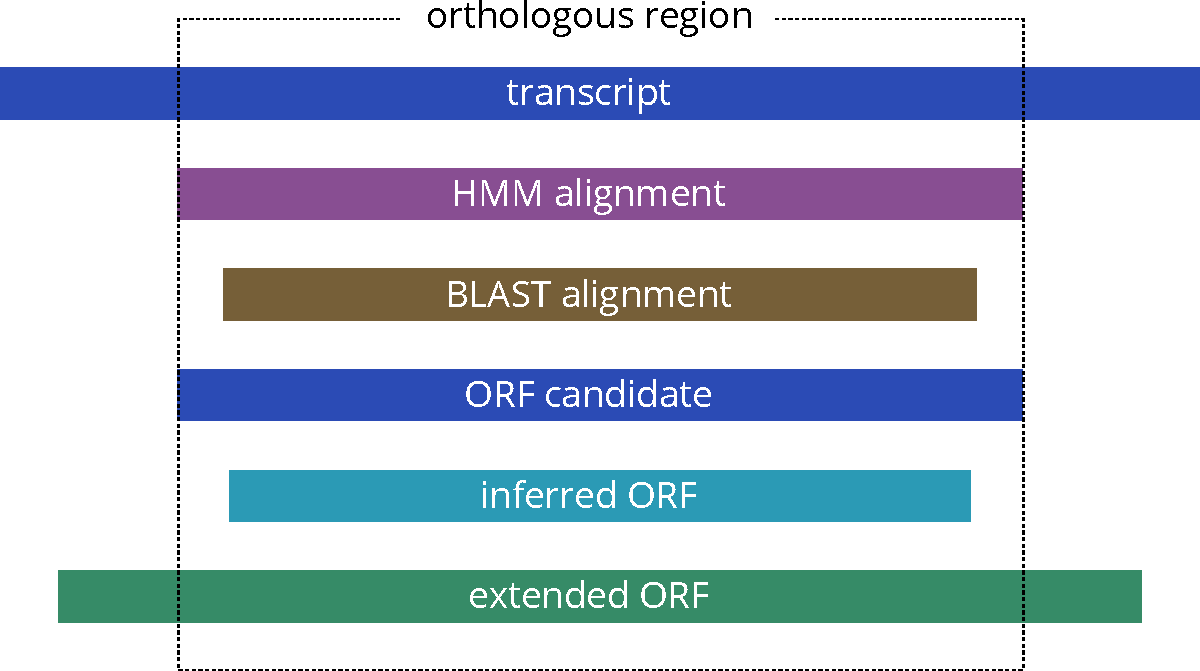
\includegraphics[width=\textwidth]{figures/alignment-regions.pdf}
\caption[Alignment regions in Orthograph]{Alignment regions in
Orthograph. On the transcript, there is a candidate ortholog region that
was identified using a HMM alignment. The reverse search result using
BLAST confirms orthology for the candidate region. For ORF inference,
the transcript subsequence that was identified as putatively orthologous
using the HMM search is used. The resulting ORF may then be extended by
using the entire transcript sequence, resulting in ORF coordinates that
exceed the orthologous region.}
\label{fig:alignment-regions}
\end{figure}

\newpage

\begin{figure}[htbp]
\centering
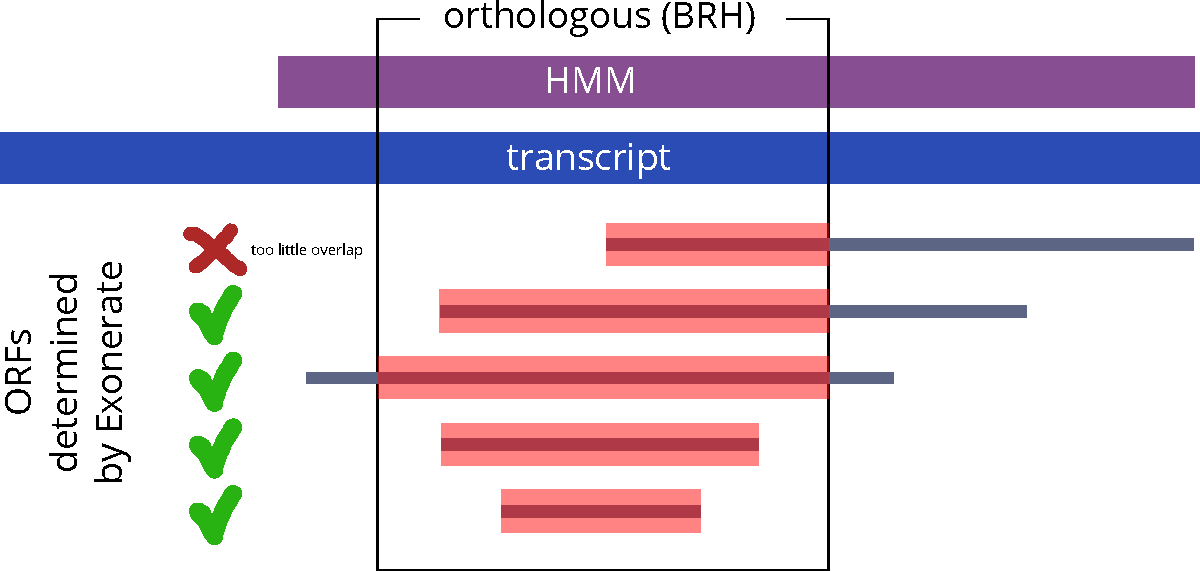
\includegraphics[width=\textwidth]{figures/orf-overlap-minimum.pdf}
\caption[ORF extension criteria in Orthograph]{ORF extension criteria in
Orthograph. Inferred ORFs that do not overlap at least 50 \% of the
orthologous region are discarded due to insufficient confidence in
orthology status. As long as the majority of the ORF length is inside
the orthologous region on the transcript, ORFs are accepted.}
\label{fig:orf-overlap}
\end{figure}

\newpage

\begin{figure}[htbp]
\centering
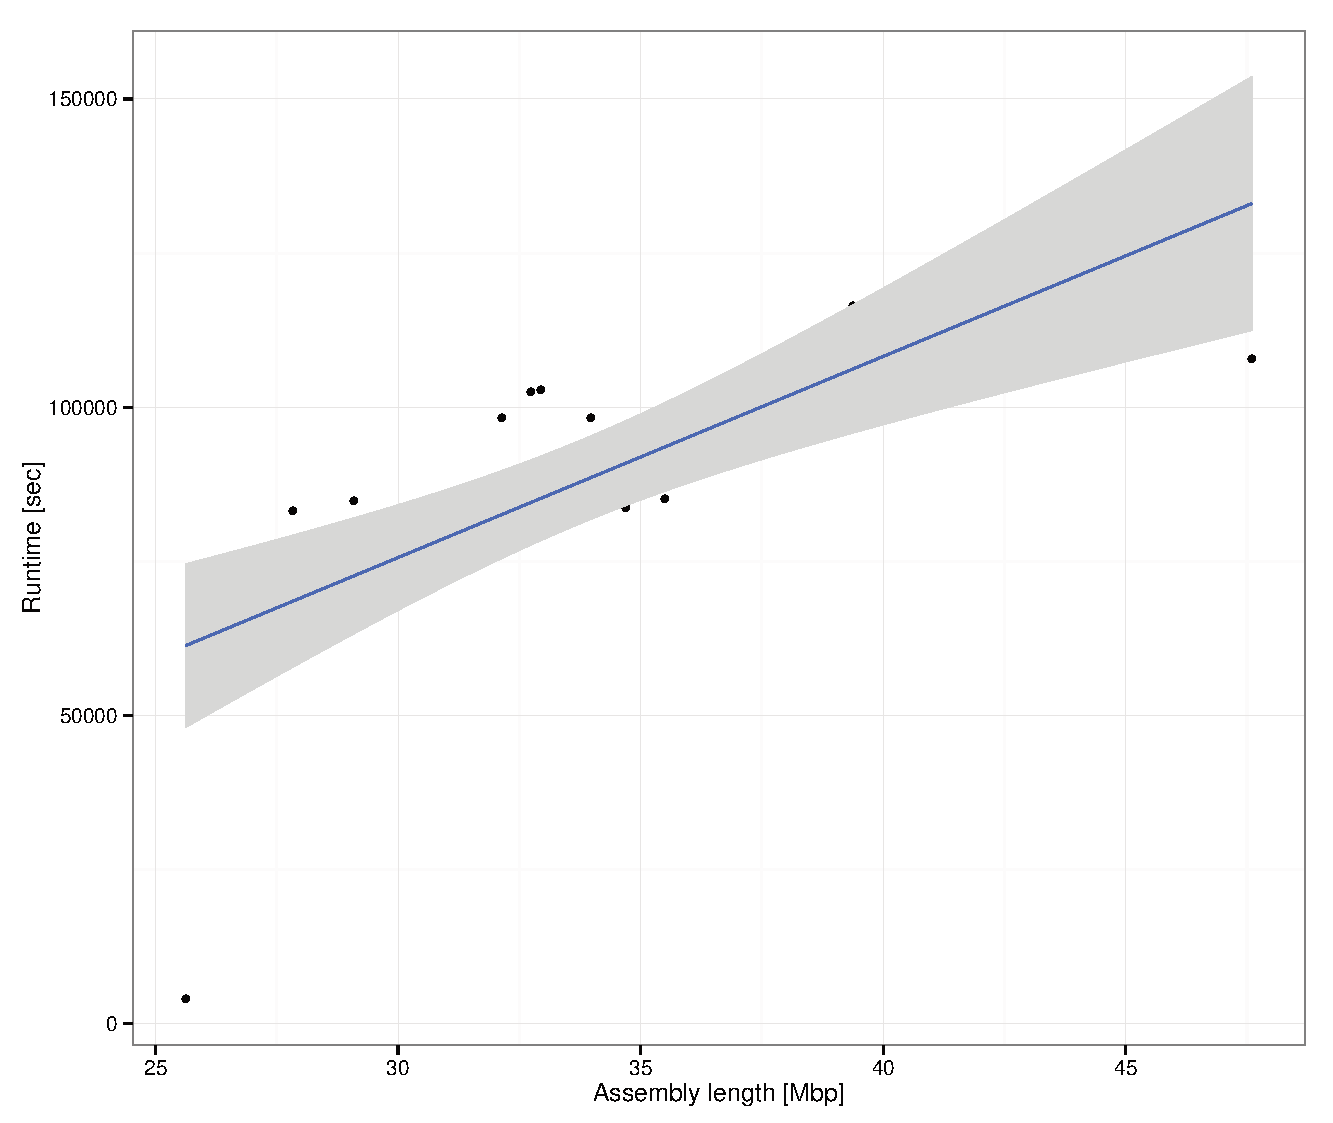
\includegraphics[width=\textwidth]{figures/runtime-vs-length.pdf}
\caption[Orthograph runtime is correlated to assembly length]{Orthograph
runtime is significantly correlated to total transcriptome assembly
length (Spearman rank correlation, $S = 326$, $p \ll 0.001$) when
running with a single thread. Dots indicate measurements for individual
transcriptome assemblies. Blue line: linear regression model; gray area:
confidence interval.}
\label{fig:runtime-vs-length}
\end{figure}

\newpage

\begin{figure}[htbp]
\centering
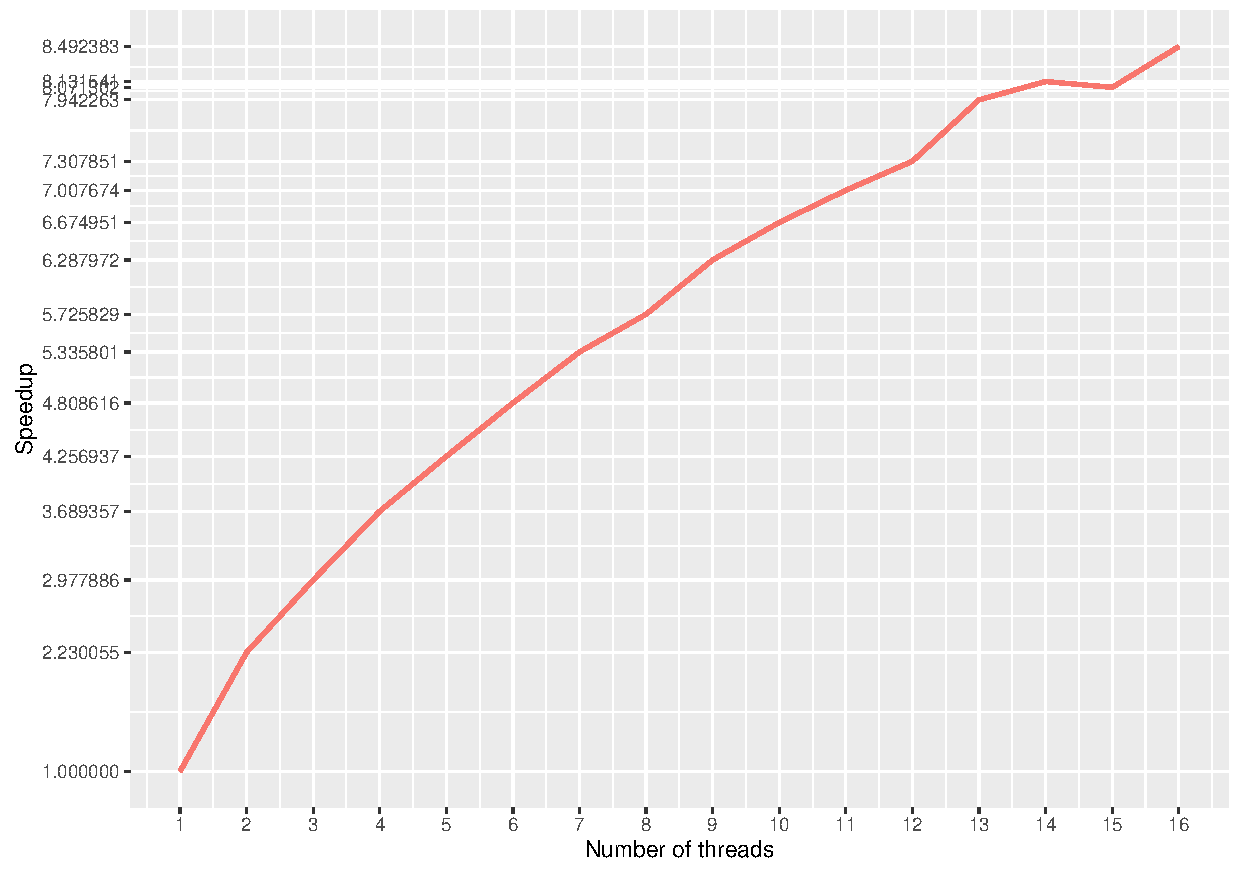
\includegraphics[width=\textwidth]{figures/runtime-speedup.pdf}
\caption[Orthograph multithreading speedup graph]{Orthograph profits
from multiple CPU threads. The x axis shows the number of CPU threads;
the y axis shows the relative speedup compared to single-threaded
performance on a transcriptome assembly of 34 Mbp. Using 16 threads
reduces Orthograph runtime to 11.7 \% of single-threaded runtime.}
\label{fig:runtime-speedup}
\end{figure}

\newpage

\begin{sidewaysfigure}
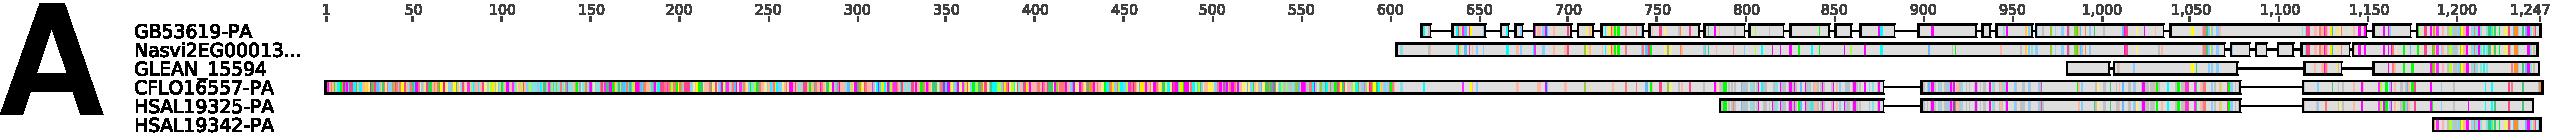
\includegraphics[height=2em]{figures/alignment-clustalw.pdf}\\
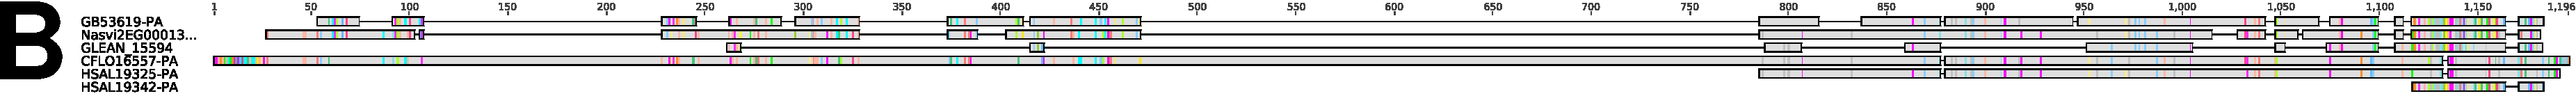
\includegraphics[height=2em]{figures/alignment-muscle.pdf}
\caption[Multiple sequence alignments of an ortholog group]{%
Multiple sequence alignment (MSA) of an ortholog group (OG) as an
examplary assignment of a gene from the \emph{H. saltator} reference
gene set (RGS) to the ``wrong'' OG.  A: Alignment using the ClustalW
algorithm \citep{Thompson1994}; B: Alignment using the MUSCLE algorithm
\citep{Edgar2004}.  According to OrthoDB, the protein HSAL19342-PA
belongs to the OG with the ID EOG7KHN7Q.  Orthograph, however,
identified the protein HSAL19325-PA as orthologous to this OG due to a
high similarity to one of the proteins in the OG (404 amino acids
alignment overlap, 64.6 \% identical sites).  The sequence HSAL19325-PA
has been added to the MSA to demonstrate that it is in large parts more
similar to a sequence from \emph{C. floridanus} (CFLO16557-PA) and
therefore yields a higher alignment bit score than the correct --
according to OrthoDB -- ortholog HSAL19342-PA.  In contrast, the protein
that is recorded in OrthoDB as part of the OG is shorter and displays
little similarity (61 amino acids alignment overlap, 31.1 \% identical
sites).  This leads to a higher bit score in the reverse search for the
longer and more similar -- but not orthologous according to OrthoDB --
sequence.  In turn, the BRH criterion for the correct, but shorter
ortholog (according to OrthoDB) was not fulfilled.  This demonstrates
that using different alignment algorithms can impede successful
orthology assignment.  Grey areas indicate conserved regions, colored
bars indicate sequence-specific different amino acid positions.  Graphic
created using Geneious v7.1 (\url{http://www.geneious.com}).}%
\label{fig:orthodb-alignments}
\end{sidewaysfigure}

\newpage

\section{Supplementary Tables}

\begin{table}[h]
\footnotesize
\centering
\caption{Species for which 1KITE transcriptomes were analyzed.}
\label{tab:species}
\begin{tabular}{@{}lllll@{}}
\toprule
Order       & Family      & Subfamily      & Genus         & Species                     \\ 
\midrule
Hymenoptera & Crabronidae & Bembicinae     & Alyssontini   & \emph{Alysson spinosus}            \\
Hymenoptera & Crabronidae & Bembicinae     & Bembicini     & \emph{Bembix rostrata}             \\
Hymenoptera & Crabronidae & Bembicinae     & Bembicini     & \emph{Gorytes laticinctus}         \\
Hymenoptera & Crabronidae & Bembicinae     & Bembicini     & \emph{Harpactus elegans}           \\
Hymenoptera & Crabronidae & Bembicinae     & Bembicini     & \emph{Sphecius convallis}          \\
Hymenoptera & Crabronidae & Bembicinae     & Bembicini     & \emph{Stizoides tridentatus}       \\
Hymenoptera & Crabronidae & Bembicinae     & Nyssonini     & \emph{Nysson niger}                \\
Hymenoptera & Crabronidae & Crabroninae    & Crabronini    & \emph{Crabro peltarius}            \\
Hymenoptera & Crabronidae & Crabroninae    & Crabronini    & \emph{Crossocerus quadrimaculatus} \\
Hymenoptera & Crabronidae & Crabroninae    & Larrini       & \emph{Tachysphex fulvitarsis}      \\
Hymenoptera & Crabronidae & Crabroninae    & Oxybelini     & \emph{Oxybelus bipunctatus}        \\
Hymenoptera & Crabronidae & Crabroninae    & Trypoxylini   & \emph{Trypoxylon figulus}          \\
Hymenoptera & Crabronidae & Dinetinae      & -             & \emph{Dinetus pictus}              \\
Hymenoptera & Crabronidae & Pemphredoninae & Pemphredonini & \emph{Diodontus minutus}           \\
Hymenoptera & Crabronidae & Pemphredoninae & Pemphredonini & \emph{Pemphredon lugens}           \\
Hymenoptera & Crabronidae & Pemphredoninae & Psenini       & \emph{Psenulus fuscipennis}        \\
Hymenoptera & Crabronidae & Philanthinae   & Cercerini     & \emph{Cerceris arenaria}           \\
Hymenoptera & Crabronidae & Philanthinae   & Philanthini   & \emph{Philanthus triangulum}       \\
Hymenoptera & Sphecidae   & Ammophilinae   & -             & \emph{Podalonia hirsuta}           \\
Hymenoptera & Sphecidae   & Sceliphrinae   & Sceliphrini   & \emph{Chalybion californicum}      \\
Hymenoptera & Sphecidae   & Sceliphrinae   & Sceliphrini   & \emph{Sceliphron curvatum}         \\
Hymenoptera & Sphecidae   & Sphecinae      & Prionychini   & \emph{Prionyx kirbii}              \\
Hymenoptera & Sphecidae   & Sphecinae      & Sphecini      & \emph{Isodontia mexicana}          \\
Hymenoptera & Sphecidae   & Sphecinae      & Sphecini      & \emph{Sphex funerarius}            \\ 
\bottomrule
\end{tabular}
\end{table}

\begin{table}[h]
\footnotesize
\centering
\caption[Orthograph requirements]{Software packages required by Orthograph. It has been developed and tested with these versions. Older versions are not supported.}
\label{tab:software}
\begin{tabular}{@{}lll@{}}
\toprule
Package     & Version & Download from \\
\midrule
Perl        & 5.14    & \url{http://www.perl.org}                                         \\
SQLite      & 3.8.2   & \url{http://sqlite.org/download.html}                             \\
MySQL       & 5.6.17  & \url{http://dev.mysql.com/downloads/mysql/}                       \\
MAFFT       & 7.023b  & \url{http://mafft.cbrc.jp/alignment/software/}                    \\
HMMer       & 3.1b1   & \url{http://hmmer.janelia.org/software/}                          \\
NCBI BLAST+ & 2.2.28+ & \url{ftp://ftp.ncbi.nlm.nih.gov/blast/executables/blast+/LATEST/} \\
Exonerate   & 2.2.0   & \url{http://www.ebi.ac.uk/~guy/exonerate/}                        \\
\bottomrule
\end{tabular}
\end{table}

\begin{sidewaystable}[h]
\footnotesize
\caption{Official gene sets for the reference ortholog set generation.}
\label{tab:ogs}
\begin{tabular}{@{}llll@{}}
\toprule
Species                         & Version  & Citation \\ \midrule
\species{Acromyrmex echinatior} & 1.2      & \citet{Nygaard2011} \\
\species{Apis mellifera}        & 1.1      & \citet{Honeybee2006} \\
\species{Atta cephalotes}       & 1.2      & \citet{Suen2011} \\
\species{Camponotus floridanus} & 3.3      & \citet{Bonasio2010} \\
\species{Harpegnathos saltator} & 3.3      & \citet{Bonasio2010} \\
\species{Linepithema humile}    & 1.2      & \citet{Smith2011a} \\
\species{Nasonia vitripennis}   & 1.2      & \citet{Werren2010} \\
\species{Tribolium castaneum}   & 3.0      & \citet{TriboliumGenomeSequencingConsortium2008} \\
\bottomrule
\end{tabular}\\
\species{Acromyrmex echinatior}: \url{http://hymenopteragenome.org/acromyrmex/?q=genome_consortium_datasets}\\
\species{Apis mellifera}       : \url{http://hymenopteragenome.org/beebase/?q=download_sequence}\\
\species{Atta cephalotes}      : \url{http://hymenopteragenome.org/atta/?q=genome_consortium_datasets}\\
\species{Camponotus floridanus}: \url{http://hymenopteragenome.org/camponotus/?q=genome_consortium_datasets}\\
\species{Harpegnathos saltator}: \url{http://hymenopteragenome.org/harpegnathos/?q=genome_consortium_datasets}\\
\species{Linepithema humile}   : \url{http://hymenopteragenome.org/linepithema/?q=genome_consortium_datasets}\\
\species{Nasonia vitripennis}  : \url{http://hymenopteragenome.org/nasonia/?q=sequencing_and_analysis_consortium_datasets}\\
\species{Tribolium castaneum}  : \url{http://beetlebase.org/?q=download_settings}
\end{sidewaystable}

% Please add the following required packages to your document preamble:
% \usepackage{booktabs}
\begin{table}[h]
\scriptsize
\caption[Species, 1KITE library IDs, NCBI accession numbers, and assembly
statistics of the apoid wasp transcriptomes that were released with the
Orthograph publication]{Species, 1KITE library IDs (see http:// 1
kite.org/ 1 kite\_species.php ), number of assembled
transcripts, total assembly size, N50 values, and NCBI GenBank accession numbers. Note that the
assemblies were filtered to contain only contigs longer than 199 bp.}
\label{tab:1kite-apoid-wasps-accessions}
\begin{tabular}{@{}lllllll@{}}
\toprule
Species                     & 1KITE library ID   & Tax. ID & BioProject & BioSample accession & Sample acc. & Exp. accession \\ \midrule
\species{Alysson spinosus}            & INSytvTBDRAAPEI-9  & 1507100     & 252289     & SAMN02870203        & SRS651858        & SRX642976            \\
\species{Bembix rostrata}             & INSswpTBNRAAPEI-44 & 1507104     & 252270     & SAMN02870220        & SRS651839        & SRX642957            \\
\species{Cerceris arenaria}           & INSytvTBFRAAPEI-12 & 1507109     & 252291     & SAMN02870235        & SRS651861        & SRX642978            \\
\species{Chalybion californicum}      & INSytvTBQRAAPEI-57 & 411700      & 252298     & SAMN02870236        & SRS651868        & SRX642985            \\
\species{Crabro peltarius}            & INSswpTBJRAAPEI-37 & 1507127     & 252268     & SAMN02870270        & SRS651838        & SRX642955            \\
\species{Crossocerus quadrimaculatus} & INSswpTBPRAAPEI-46 & 1126388     & 252271     & SAMN02870271        & SRS651841        & SRX642958            \\
\species{Dinetus pictus}              & INSjdsTAYRAAPEI-43 & 1507342     & 252320     & SAMN02870280        & SRS651890        & SRX643007            \\
\species{Diodontus minutus}           & INSjdsTBMRAAPEI-88 & 1294192     & 252322     & SAMN02870281        & SRS651892        & SRX643009            \\
\species{Gorytes laticinctus}         & INSytvTBERAAPEI-11 & 1126390     & 252290     & SAMN02870305        & SRS651860        & SRX642977            \\
\species{Harpactus elegans}           & INSswpTAFRAAPEI-16 & 1507137     & 252247     & SAMN02870308        & SRS651818        & SRX642935            \\
\species{Isodontia mexicana}          & INSswpTBDRAAPEI-30 & 288402      & 252264     & SAMN02870321        & SRS651834        & SRX642951            \\
\species{Nysson niger}                & INSswpTBGRAAPEI-34 & 1507151     & 252266     & SAMN02870351        & SRS651836        & SRX642953            \\
\species{Oxybelus bipunctatus}        & INSjdsTBIRAAPEI-75 & 1507154     & 252321     & SAMN02870362        & SRS651891        & SRX643008            \\
\species{Pemphredon lugens}           & INSytvTBBRAAPEI-95 & 1507158     & 252288     & SAMN02870371        & SRS651859        & SRX642975            \\
\species{Philanthus triangulum}       & INSswpTBTRABPEI-62 & 280486      & 252273     & SAMN02870374        & SRS651843        & SRX642960            \\
\species{Podalonia hirsuta}           & INSswpTBRRAAPEI-56 & 1088627     & 252272     & SAMN02870381        & SRS651842        & SRX642959            \\
\species{Prionyx kirbii}              & INSytvTBSRAAPEI-74 & 330847      & 252299     & SAMN02870385        & SRS651869        & SRX642986            \\
\species{Psenulus fuscipennis}        & INSswpTATRAAPEI-13 & 1507163     & 252256     & SAMN02870386        & SRS651827        & SRX642944            \\
\species{Sceliphron curvatum}         & INSswpTAZRAAPEI-19 & 1507168     & 252261     & SAMN02870396        & SRS651832        & SRX642949            \\
\species{Sphecius convallis}          & INSnfrTBORAAPEI-14 & 420963      & 252349     & SAMN02870401        & SRS651919        & SRX643036            \\
\species{Sphex funerarius}            & INSytvTAIRAAPEI-18 & 1507169     & 252279     & SAMN02870403        & SRS651849        & SRX642966            \\
\species{Stizoides tridentatus}       & INSytvTARRAAPEI-44 & 1507174     & 252284     & SAMN02870412        & SRS651854        & SRX642971            \\
\species{Tachysphex fulvitarsis}      & INSswpTAKRAAPEI-21 & 1507176     & 252251     & SAMN02870419        & SRS651822        & SRX642939            \\
\species{Trypoxylon figulus}          & INSytvTAWRAAPEI-88 & 1124897     & 252286     & SAMN02870436        & SRS651856        & SRX642973            \\ \bottomrule
\end{tabular}

\bigskip

\begin{tabular}{@{}lllllll@{}}
\toprule
Species                     & Run accession & TSA project accession & TSA version  & Transcripts & Total length & N50   \\ \midrule
\species{Alysson spinosus}            & SRR1503092    & GBUA00000000          & GBUA01000000 & 40,680      & 47,606,733   & 1,568 \\
\species{Bembix rostrata}             & SRR1503073    & GBQR00000000          & GBQR01000000 & 33,341      & 37,839,804   & 6,031 \\
\species{Cerceris arenaria}           & SRR1503094    & GBNS00000000          & GBNS01000000 & 24,719      & 34,252,864   & 3,305 \\
\species{Chalybion californicum}      & SRR1503101    & GBOM00000000          & GBOM01000000 & 21,323      & 33,977,878   & 3,834 \\
\species{Crabro peltarius}            & SRR1503071    & GBWG00000000          & GBWG01000000 & 17,826      & 27,839,732   & 4,932 \\
\species{Crossocerus quadrimaculatus} & SRR1503074    & GBWH00000000          & GBWH01000000 & 16,354      & 27,670,170   & 5,280 \\
\species{Dinetus pictus}              & SRR1503123    & GBLS00000000          & GBLS01000000 & 20,195      & 35,261,360   & 5,479 \\
\species{Diodontus minutus}           & SRR1503125    & GBMA00000000          & GBMA01000000 & 22,820      & 39,373,028   & 3,107 \\
\species{Gorytes laticinctus}         & SRR1503093    & GBNR00000000          & GBNR01000000 & 20,336      & 30,119,789   & 7,540 \\
\species{Harpactus elegans}           & SRR1503051    & GBNF00000000          & GBNF01000000 & 22,245      & 35,499,888   & 4,814 \\
\species{Isodontia mexicana}          & SRR1503067    & GBPY00000000          & GBPY01000000 & 34,622      & 38,000,489   & 2,600 \\
\species{Nysson niger}                & SRR1503069    & GBNN00000000          & GBNN01000000 & 22,496      & 29,091,955   & 4,151 \\
\species{Oxybelus bipunctatus}        & SRR1503124    & GBLU00000000          & GBLU01000000 & 22,233      & 37,187,137   & 2,311 \\
\species{Pemphredon lugens}           & SRR1503091    & GBQH00000000          & GBQH01000000 & 24,675      & 39,425,911   & 716   \\
\species{Philanthus triangulum}       & SRR1503076    & GBWI00000000          & GBWI01000000 & 21,735      & 27,360,360   & 4,209 \\
\species{Podalonia hirsuta}           & SRR1503075    & GBPX00000000          & GBPX01000000 & 21,108      & 32,136,789   & 4,075 \\
\species{Prionyx kirbii}              & SRR1503102    & GBQI00000000          & GBQI01000000 & 21,703      & 31,095,319   & 8,540 \\
\species{Psenulus fuscipennis}        & SRR1503060    & GBNH00000000          & GBNH01000000 & 24,423      & 31,095,907   & 1,024 \\
\species{Sceliphron curvatum}         & SRR1503065    & GBNL00000000          & GBNL01000000 & 22,934      & 32,739,311   & 6,440 \\
\species{Sphecius convallis}          & SRR1503152    & GBOB00000000          & GBOB01000000 & 19,967      & 25,618,375   & 3,922 \\
\species{Sphex funerarius}            & SRR1503082    & GBQD00000000          & GBQD01000000 & 26,189      & 37,503,328   & 1,476 \\
\species{Stizoides tridentatus}       & SRR1503087    & GBQO00000000          & GBQO01000000 & 27,724      & 34,689,230   & 5,790 \\
\species{Tachysphex fulvitarsis}      & SRR1503055    & GBPR00000000          & GBPR01000000 & 17,308      & 32,940,922   & 8,852 \\
\species{Trypoxylon figulus}          & SRR1503089    & GBWO00000000          & GBWO01000000 & 19,174      & 31,640,527   & 4,800 \\ \bottomrule
\end{tabular}
\end{table}

\newpage
